\subsection{Implementation approaches}

Apart from the theoretical analysis, this thesis work also considers two different implementations of systems, similar to Blocket Secure Package, which is described in previous section. The two systems in question are implemented, using different approaches and architectures, however, despite the differences in implementation strategy, their initial goal was to provide roughly the same functionality. This section provides a rough description of those two approaches.

\begin{figure}[H]
\centering
\begin{subfigure}{.478\textwidth}
\centering
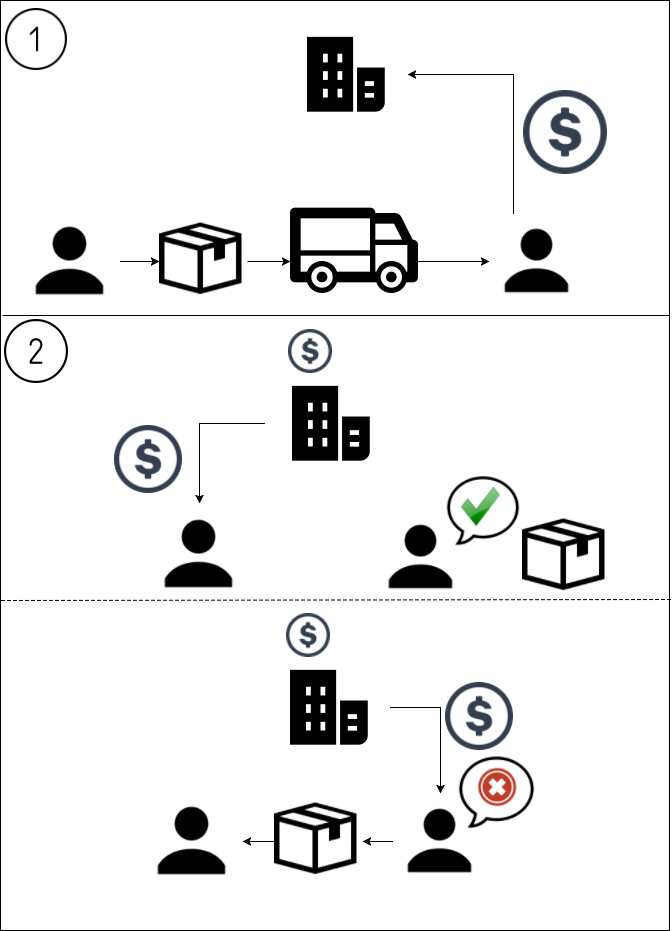
\includegraphics[width=.9\linewidth]{images/originalservice.png}
\caption{Centralized implementation.}
\label{fig:orig}
\end{subfigure}%
\begin{subfigure}{.435\textwidth}
\centering
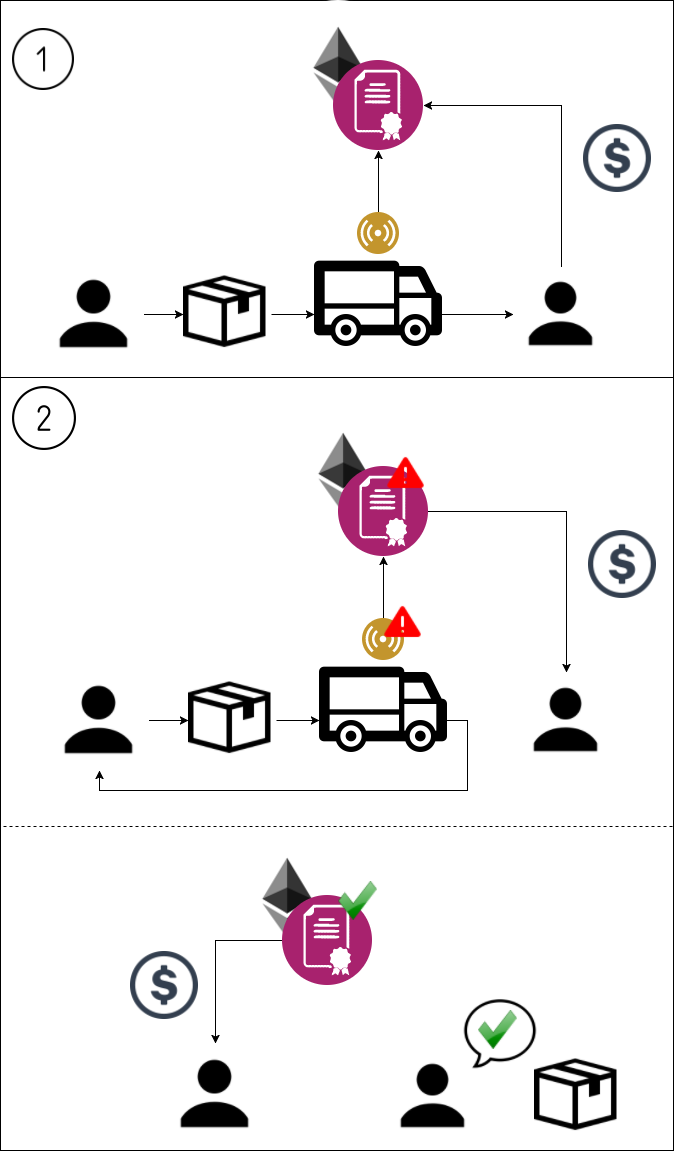
\includegraphics[width=.8\linewidth]{images/proposedservice.png}
\caption{Decentralized implementation.}
\label{fig:prop}
\end{subfigure}
\caption{Illustration of the implementation approaches.}
\label{fig:test}
\end{figure}

\subsubsection{Decentralized approach} \label{section:decentralizedapproach}

This version of the Secure Package system was implemented by fellow master thesis student, Axel Vallin, as his own separate thesis work. It was developed on an instance of Ethereum blockchain and uses smart contracts for the storage and transfer of data. Payments are processed, using the customized ERC20 tokens \citep{erc20}, which will be stored in the smart contract, before moving to sellers account, as illustrated in Figure \ref{fig:prop} (assuming that the buyer is satisfied with the condition of goods). These ERC20 tokens have a potential to be converted to \emph{\gls{fiat money}} by either implementing an internal exchange mechanism of some sort, which would probably require the issuance of an Initial Coin Offering (ICO) \citep{ico}, or the registration of the tokens on an external cryptocurrency exchange, where it could be traded to fiat money and other cryptocurrencies. A partially-automated system for conflict resolving (when the actors disagree about the condition of goods, or if the parcel gets damaged during the transfer) is to be implemented. Support for sensors, which can be attached to the parcel, such as accelerometers, pressure sensors and GPS is added (more detailed discussion about the sensors is provided in Section \ref{section:improvementsfromoriginal}). The application is accessed though a web interface. More details, regarding the decentralized implementation and its development process, can be found in the master thesis report by Axel Vallin \citep{axelrapport}.

One of the main reasons for implementing the system, using blockchain, is to eliminate the third party aspect and potential security flaws regarding it (detailed discussion on that topic is provided in Section \ref{section:analysisthirdparty}). Other quality attributes, such as security, reusability, data integrity etc. may, in theory, be improved, using this implementation method.



\subsubsection{Traditional approach with blockchain influence} \label{section:centralizedapproach}
This version was designed and implemented as part of this thesis work. It was built, using the client-server architecture in general. All of the personal data, public encryption keys and transactions are stored in a database. Payments are simulated using fiat currency (payment alternative, using the same ERC20 token as in the decentralized version is an additional goal) and funds are stored in the hands of a third party during the transfer of goods, just like in the original system by Blocket, as was illustrated in Figure \ref{fig:orig}. However, some additional functionality is implemented. Partial transparency is integrated, so that anyone can gain access to the central database and access unencrypted data fields (to achieve similar functionality, as in the blockchain model). Same sort of sensor support, as in the decentralized implementation, is added and handled through a central server interface. An automated alert system is created, that closely monitors sensor data during the transportation of the parcel. A lot of effort was put into protecting the data from the outsiders, despite the transparency of the database, even from the clerk administrators, which are used for conflict resolving. Detailed discussion, regarding the implementation process of centralized system and its features is provided in Section \ref{section:design}.

The major point of this system is to provide the users with a more trusted centralized system, which possesses some beneficial features from blockchain environment and is, in some important aspects, better then the original Blocket Secure Package system.